\documentclass[paper=a4, fontsize=11pt, abstract=on]{scrartcl} % A4 paper and 11pt font size
\usepackage[left=2.5cm,top=2.5cm,right=2.5cm,bottom=2.5cm]{geometry} 
\usepackage{amsmath}
\usepackage[toc,page]{appendix}
\usepackage{graphicx}
\usepackage{sectsty}
\usepackage{amsfonts}
\usepackage{bbold}
\usepackage{fancyhdr}
\pagestyle{fancyplain}
\usepackage{parskip}
\usepackage{subcaption}
\usepackage{wrapfig}
\usepackage[english]{babel}
\usepackage{bibentry}
\usepackage {natbib}
\usepackage{float}
\usepackage{hyperref}
\usepackage{listings}
  \usepackage{courier}
\usepackage{graphics}
 \usepackage{color} 
 \lstset{
         basicstyle=\footnotesize\ttfamily, % Standardschrift
         %numbers=left,               % Ort der Zeilennummern
         numberstyle=\tiny,          % Stil der Zeilennummern
         %stepnumber=2,               % Abstand zwischen den Zeilennummern
         numbersep=5pt,              % Abstand der Nummern zum Text
         tabsize=2,                  % Groesse von Tabs
         extendedchars=true,         %
         breaklines=true,            % Zeilen werden Umgebrochen
         keywordstyle=\color{red},
    		frame=b,         
 %        keywordstyle=[1]\textbf,    % Stil der Keywords
 %        keywordstyle=[2]\textbf,    %
 %        keywordstyle=[3]\textbf,    %
 %        keywordstyle=[4]\textbf,   \sqrt{\sqrt{}} %
         stringstyle=\color{white}\ttfamily, % Farbe der String
         showspaces=false,           % Leerzeichen anzeigen ?
         showtabs=false,             % Tabs anzeigen ?
         xleftmargin=17pt,
         framexleftmargin=17pt,
         framexrightmargin=5pt,
         framexbottommargin=4pt,
         %backgroundcolor=\color{lightgray},
         showstringspaces=false      % Leerzeichen in Strings anzeigen ?        
 }
 \lstloadlanguages{% Check Dokumentation for further languages ...
         %[Visual]Basic
         %Pascal
         C
         %Python
         %C++
         %XML
         %HTML
         %Java
 }
\usepackage{caption}
\DeclareCaptionFont{white}{\color{white}}
\DeclareCaptionFormat{listing}{\colorbox[cmyk]{0.43, 0.35, 0.35,0.01}{\parbox{\textwidth}{\hspace{15pt}#1#2#3}}}
\captionsetup[lstlisting]{format=listing,labelfont=white,textfont=white, singlelinecheck=false, margin=0pt, font={bf,footnotesize}}



\numberwithin{equation}{section}
\numberwithin{figure}{section} 
\numberwithin{table}{section}
%\setlength\parindent{0pt}

\fancyhead[R]{\thepage} 
\fancyhead[L]{Reyes, Adam} 
\fancyhead[C]{ADI} 
\fancyfoot[L]{} 
\fancyfoot[C]{} 
\fancyfoot[R]{} 

\newcommand{\horrule}[1]{\rule{\linewidth}{#1}}

\title{	
2-D ADI Code
\horrule{0.5pt}
\normalfont \normalsize 
\textsc{Computational Physics}
}

\author{Adam Reyes} % Your name

\date{\normalsize\today} % Today's date or a custom date


\begin{document}
\maketitle

\section{Introduction}
\label{sec:intro}

We have already discussed using stable implicit methods to solve one-dimensional problems, such as the Crank-Nicolson method that is second-order in space in time. The Crank-Nicolson method can be easily generalized to two-dimensions, but now the matrix that has to be inverted in two-dimensions is much more complicated. What we can do is use an \emph{Alternating Direction Implicit}(ADI) method to advance a system in time. If we have that the time-evolution can be described by the sum of $n$ operators $L_i$ acting on our system, $u$, such as
\begin{equation}
  \label{eq:system}
  \frac{\partial u}{\partial t} = (L_1 + L_2 + ... + L_n)u
\end{equation}
then we can advance our system in $n$ time steps, where each step is implicit only in one operator $L_i$, and explicit in the others. We will approximate the time derivatives over a step of size $h$ as
\begin{equation}
  \label{eq:timeD}
  \frac{\partial u}{\partial t} = \frac{u^{m+1}-u^m}{h}
\end{equation}
The skeleton for our method then looks like
\begin{align}
  \label{eq:adi}
  \begin{split}
    \frac{u^{m+1/n}- u^m}{h/n} =& L_1u^{m+1/n} + (L_2 + ... L_n)u^m\\
    &\vdots\\
    \frac{u^{n+1}- u^{m+\frac{n-1}{n}}}{h/n} =& (L_1 + ... + L_{n-1})u^{m+\frac{n-1}{n}} + L_nu^{m+1}
  \end{split}
\end{align}
It turns out that for stability it is only necessary to advance the system implicitly for operators with the highest order spatial-derivative\cite{numerical}. 

\section{The Heat Equation}
\label{sec:heat}

The heat equation is given in cartesian coordinates by
\begin{equation}
  \label{eq:heat}
  \frac{\partial u}{\partial t} =
  \left(
    \frac{\partial ^2}{\partial x ^2} + \frac{\partial ^2}{\partial y ^2}
  \right)u
\end{equation}

So our ADI method(Eq.~\ref{eq:adi}) will be broken into two steps looks like
\begin{align}
\label{eq:heatadi}
  \begin{split}
    \frac{u^{n+1/2}-u^n}{h/2} =& D^2_xu^{n+1/2} + D^2_yu^n \\ 
    \frac{u^{n+1}-u^{n+1/2}}{h/2} =& D^2_xu^{n+1/2} + D^2_yu^{n+1}
  \end{split}
\end{align}
Where $D^2$ is the second-order space centered numerical derivative:
\begin{equation}
  \label{eq:D2}
  D^2u_i = \frac{1}{\Delta ^2}(u_{i+1} - 2u_i + u_{i-1})
\end{equation}
where $\Delta$ is the spacing between the $u_i$'s. We can see from Equations~\ref{eq:heatadi} and~\ref{eq:D2} that each time step is broken up to essentially two one-dimensional problems, where we only have to invert one matrix, of the form
\begin{equation}
  \label{eq:matrix}
  \mathbb{1}-\frac{h}{2}D^2
\end{equation}
,which is tri-diaganol and relatively simple to invert. 


\begin{figure}
  \centering
  \begin{subfigure}[b]{0.65\textwidth}
    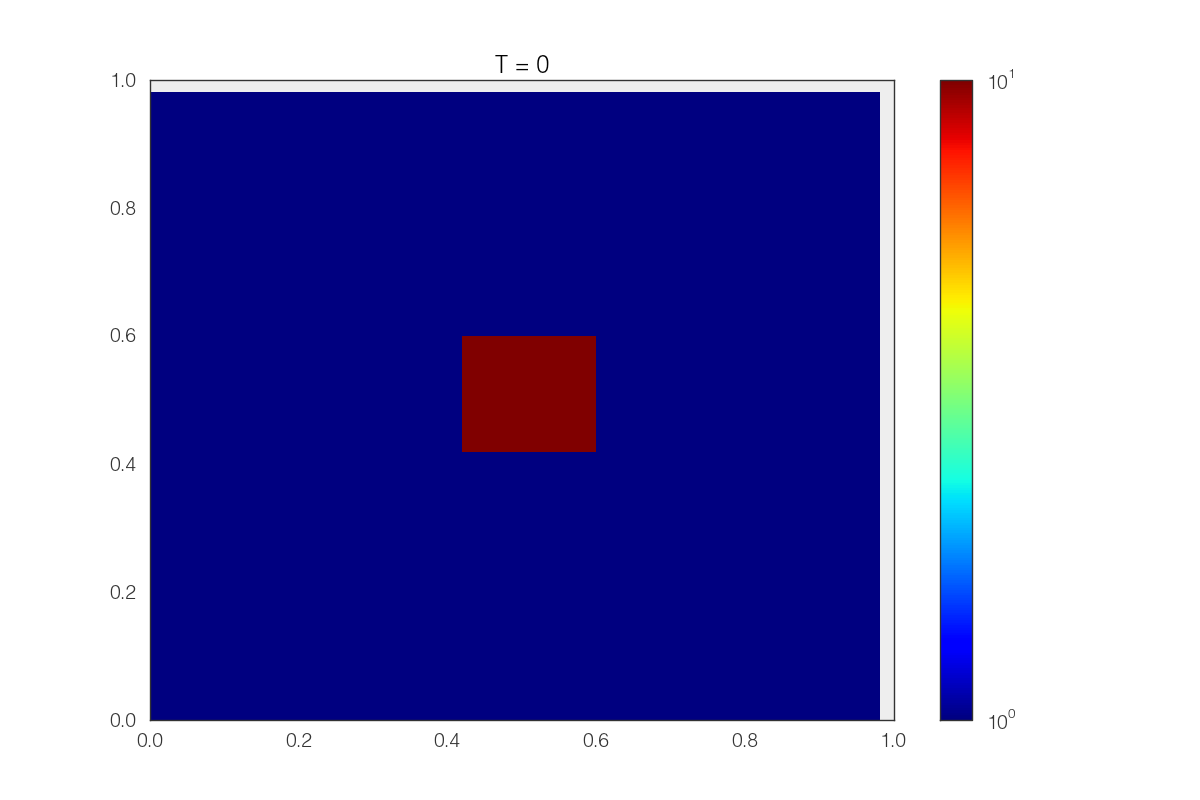
\includegraphics[width=\textwidth]{heat0}
    \caption{Initial conditions}
    \label{fig:heatinit}
  \end{subfigure}
 ~ %add desired spacing between images, e. g. ~, \quad, \qquad etc.
 % (or a blank line to force the subfigure onto a new line)
 \begin{subfigure}[b]{0.65\textwidth}
   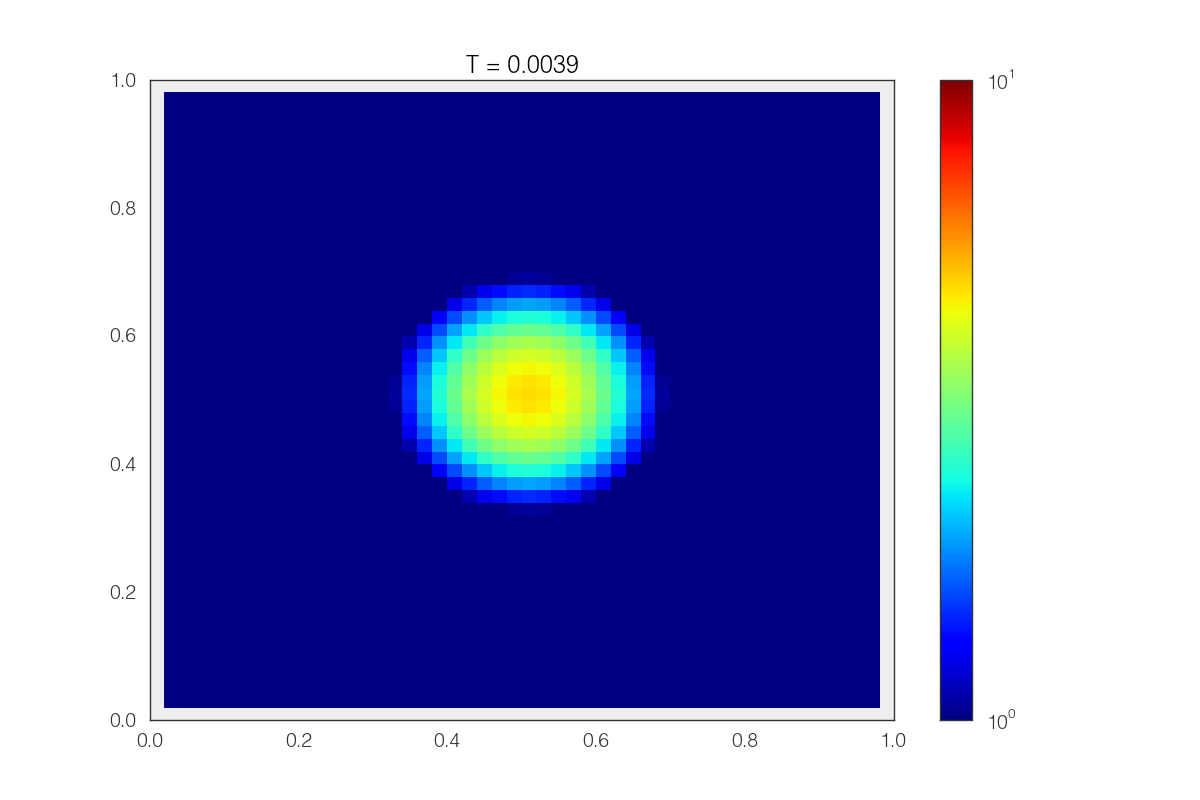
\includegraphics[width=\textwidth]{heatlong}
   \caption{Heat diffusion after some time}
   \label{fig:heatlong}
 \end{subfigure}
 \label{fig:heat}
     \caption{ADI solution to the heat equation(\ref{eq:heat}) for a 50x50 grid. See Listing~\ref{heatcode}}
\end{figure}

We can test our ADI code by solving the heat equation. I have chosen initial conditions of a square of amplitude 10 and 0 every where else(Fig. \ref{fig:heatinit}). We expect that $u$ would diffuse out evenly in all directions, which is exactly what we see in Figure~\ref{fig:heatlong}. 

\section{Laplace Equation} 
\label{sec:laplace}

Suppose our system has no time dependence, then we are left with the Laplace Equation:
\begin{equation}
  \label{eq:lap}
  \left(
    \frac{\partial ^2}{\partial x ^2} + \frac{\partial ^2}{\partial y ^2}
  \right)u = 0
\end{equation}

We can now use the method of Section~\ref{sec:heat} to relax the system in \emph{phony} time to a steady state. This is accomplished by advancing the system from a guess in \emph{time}, subject to some boundary conditions, until the additional step changes the system by some amount less than some tolerance. 
%3104771081
\begin{figure}
  \centering
  \begin{subfigure}[b]{0.65\textwidth}
    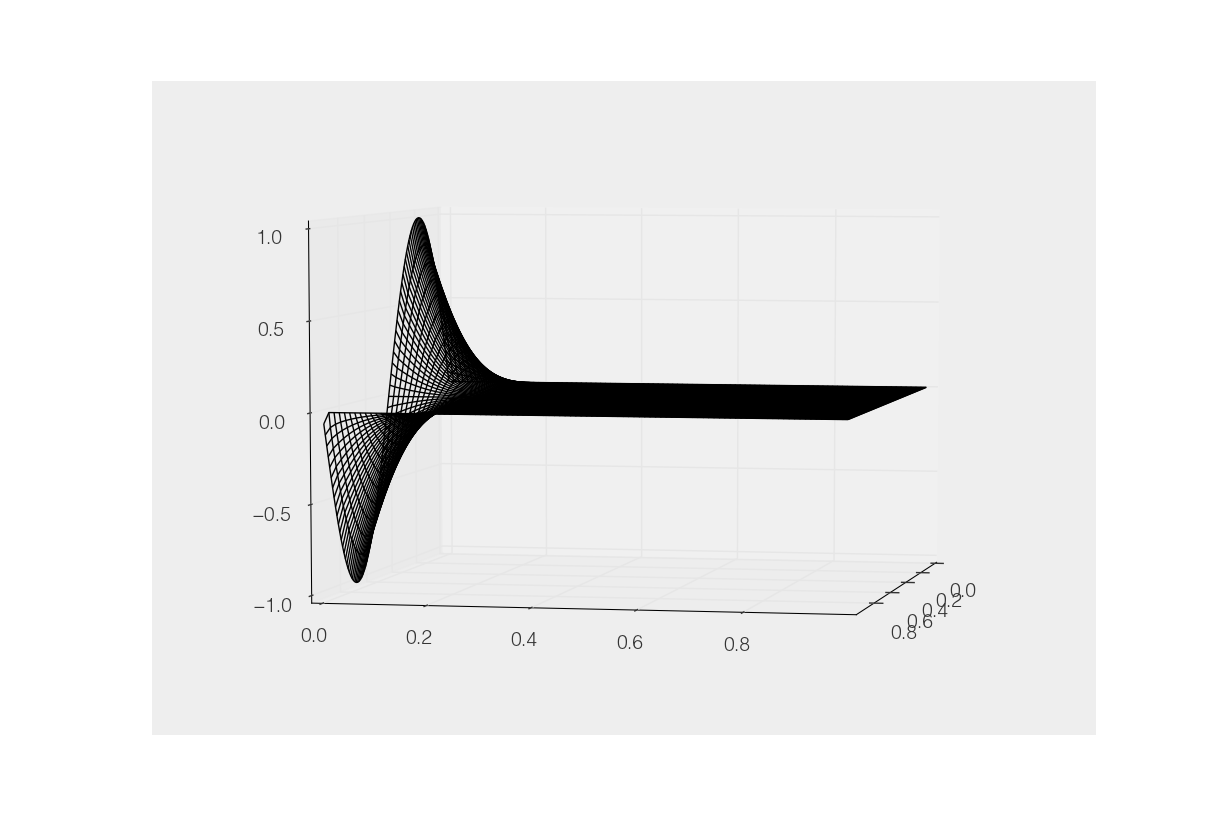
\includegraphics[width=\textwidth]{laplace}
    \label{fig:lap1}
  \end{subfigure}
  ~
  \begin{subfigure}[b]{0.65\textwidth}
    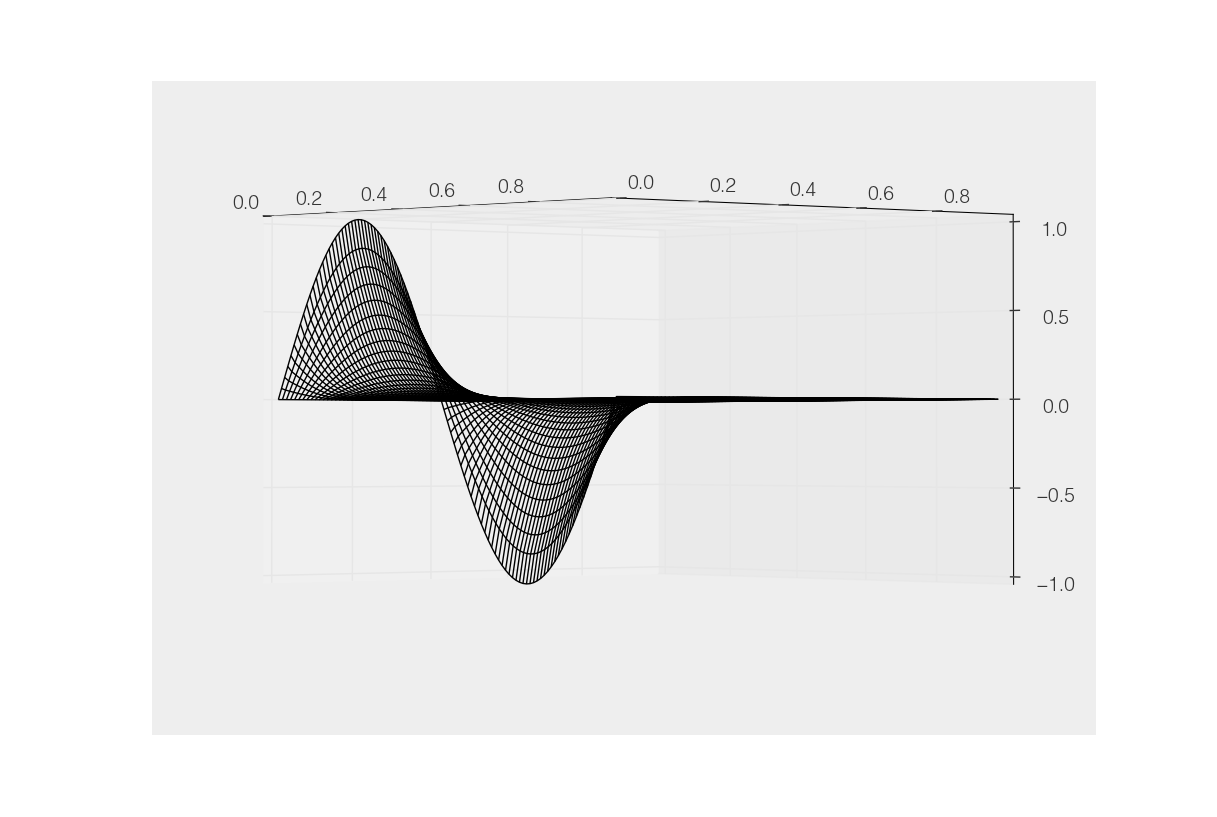
\includegraphics[width=\textwidth]{laplace2}
    \label{fig:lap2}
  \end{subfigure}
  \caption{Solution to Laplace Equation with sinusoidal boundary conditions along one end, zero others. 50x50 grid. See Listing~\ref{lapcode}}
  \label{fig:lap}
\end{figure}

To test the code for relaxing solutions to the Laplace Equation(\ref{eq:lap}) I have chosen a guess that is 1 everywhere, with boundary conditions that are sinusoidal along one boundary and zero else. Figure~\ref{fig:lap} shows that we get the solution we expect from the analytic solution, that is decaying away from the sinusoidal side as a hyperbolic trig function.

\section{Schr\"{o}dinger Equation}
\label{sec:schrod}

The Schr\"{o}dinger Equation is essentially the heat equation(\ref{eq:heat}) with an additional potential term:
\begin{equation}
  \label{eq:schrod}
  i\frac{\partial \psi}{\partial t} + \frac{\partial^2 \psi}{\partial x^2} + \frac{\partial^2 \psi}{\partial y^2} + V(x,y)\psi = 0
\end{equation}
so with a little work our method to solve the heat equation can be adapted to solve the Schr\"{o}dinger Equation. For this case our potential, $V$, does not depend on time, so there is no need to advance it explicitly, so we can incorporate it into the explicit advancement already in our method. 


\begin{figure}
  \centering
  \begin{subfigure}[b]{0.65\textwidth}
    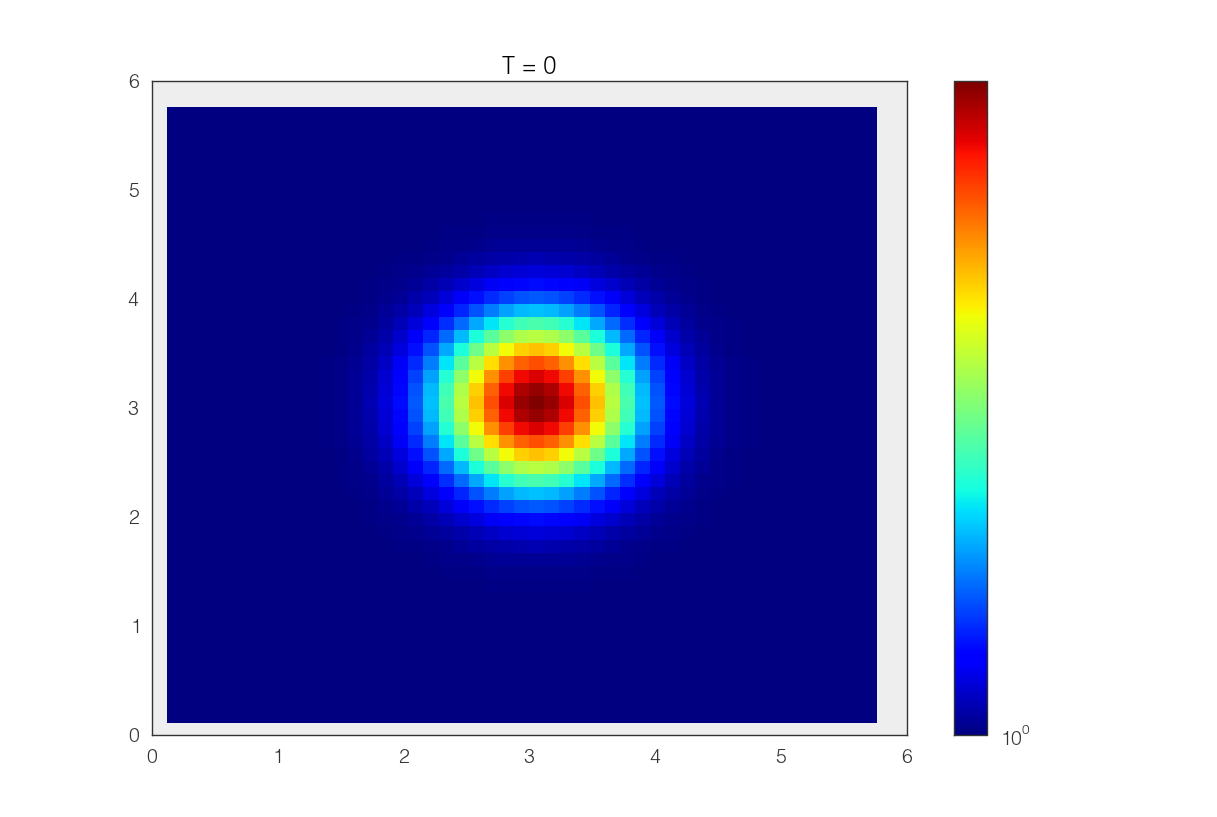
\includegraphics[width=\textwidth]{T00}
    \label{fig:harm1}
  \end{subfigure}
  ~
  \begin{subfigure}[b]{0.65\textwidth}
    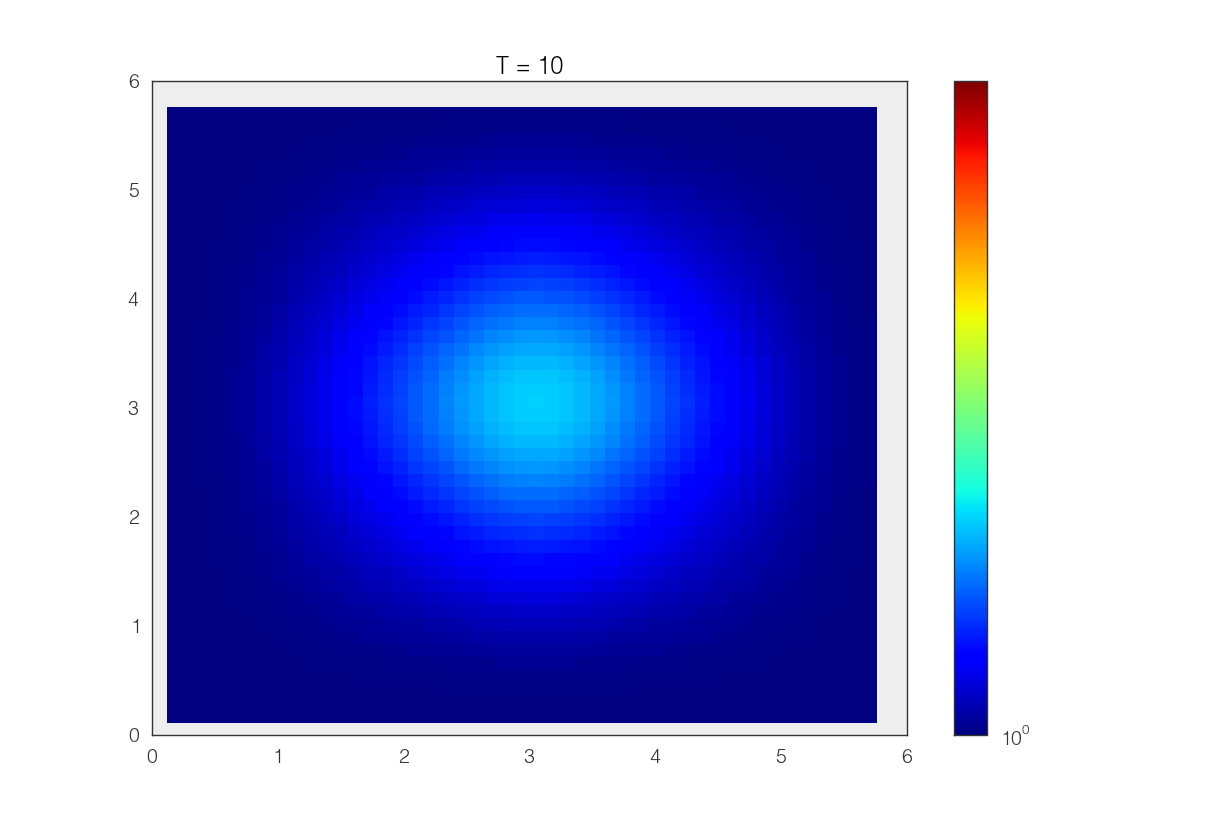
\includegraphics[width=\textwidth]{T10}
    \label{fig:harm2}
  \end{subfigure}
  \caption{Time evolution of a gaussian centered in a 2-D harmonic oscillator potential. 50x50 grid, see Listing~\ref{schrodcode}}
  \label{fig:harm}
\end{figure}

To test the method for solving the Schr\"{o}dinger Equation, we consider the two-dimensional harmonic oscillator potential given by
\begin{equation}
  \label{eq:harm}
  V(x,y) = x^2 + y^2
\end{equation}
We know that the ground state of the harmonic oscillator is a centered gaussian\cite{griff}. If we begin with a gaussian initial wavefunction, then with time we expect that the width of the gaussian profile increases and the amplitude to fall with it, to maintain the initial normalization. This is exactly what we see in Figure~\ref{fig:harm}. We also know that the first excited state is degenerate with a single node along one of the coordinate directions. I introduce a perturbation to the initial conditions of Figure~\ref{fig:harm} by multiplying by a factor proportional to $\sin y$. We would expect in time the wavefunction would start to settle into the first excited state of the harmonic oscillator. That is that the wavefunction is the same as the ground state along $x$, but goes like $e^{-y^2/2}$ along $y$. We see this happening in Figure~\ref{fig:pert}


\begin{figure}
  \centering
  \begin{subfigure}[b]{0.48\textwidth}
    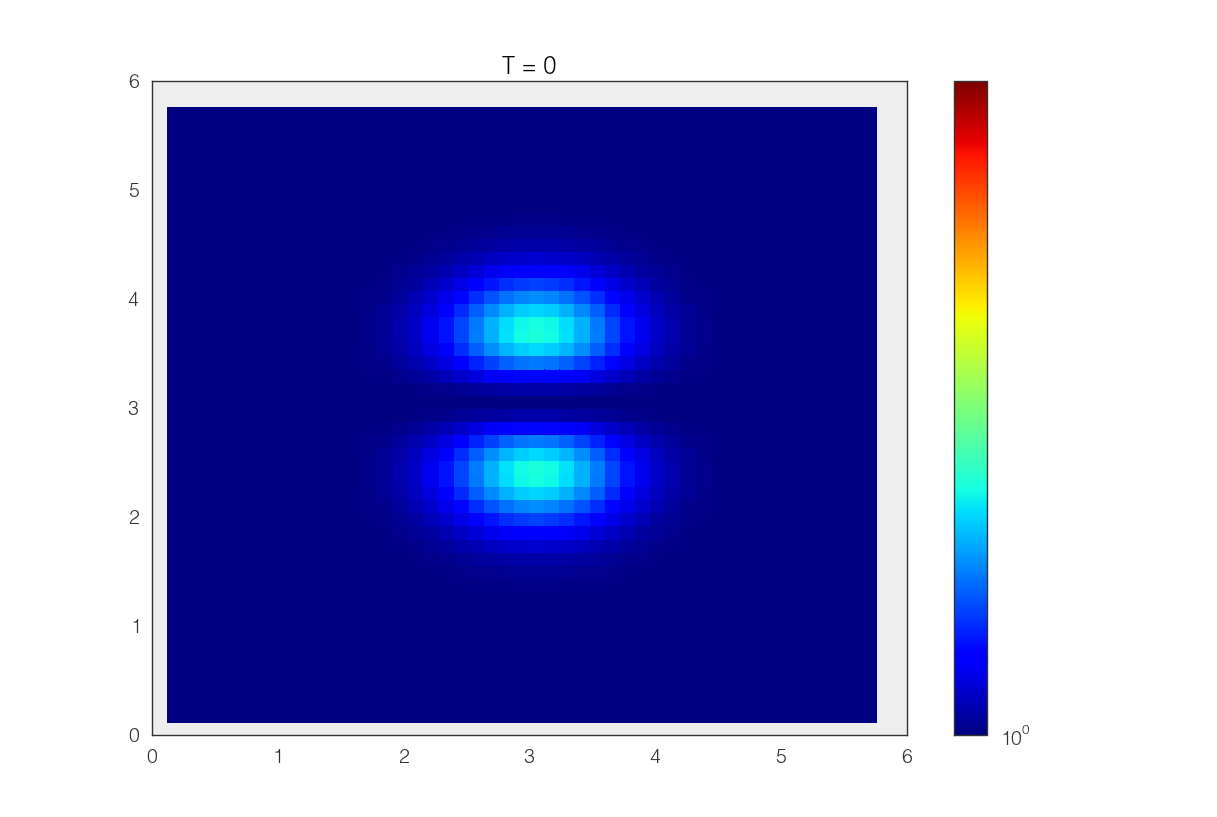
\includegraphics[width=\textwidth]{pertinit}
    \caption{}
    \label{fig:pert1}
  \end{subfigure}
  ~
  \begin{subfigure}[b]{0.48\textwidth}
    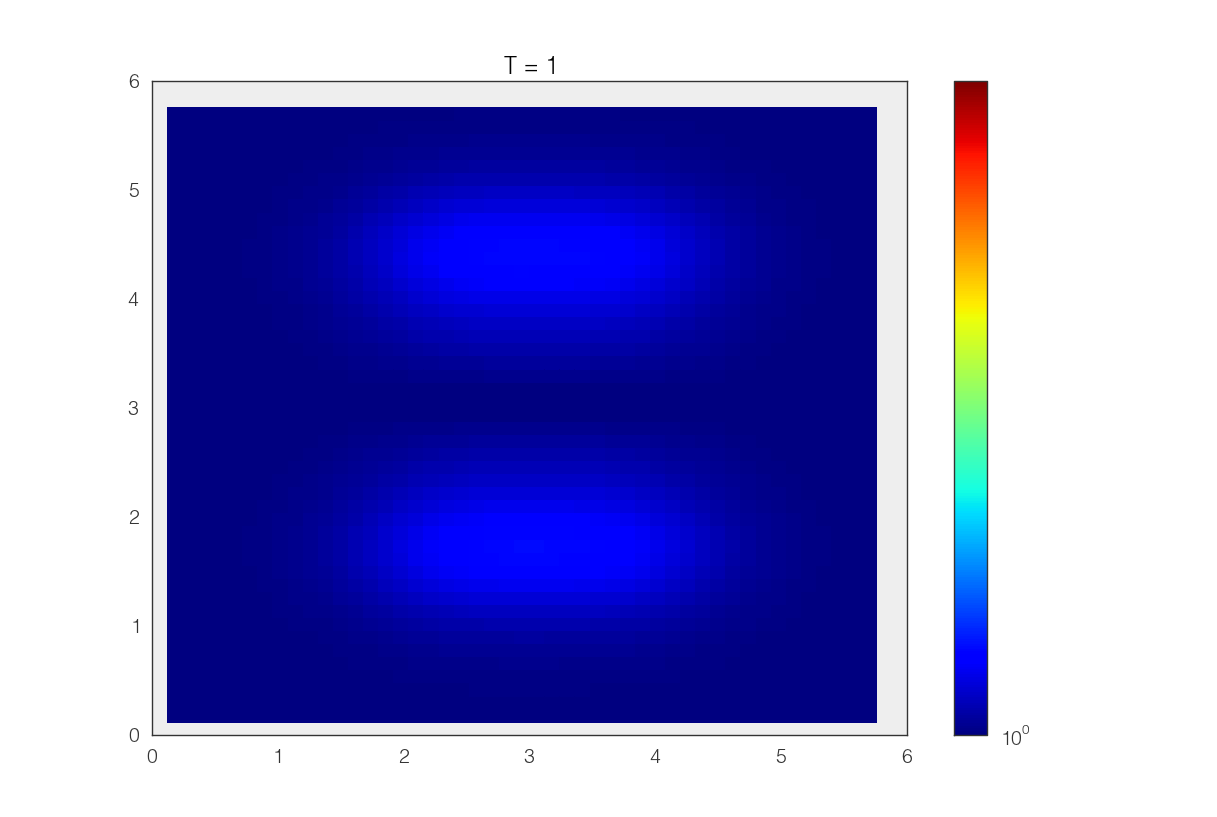
\includegraphics[width=\textwidth]{pert1}
    \caption{}
    \label{fig:pert2}
  \end{subfigure}
\begin{subfigure}[b]{0.48\textwidth}
    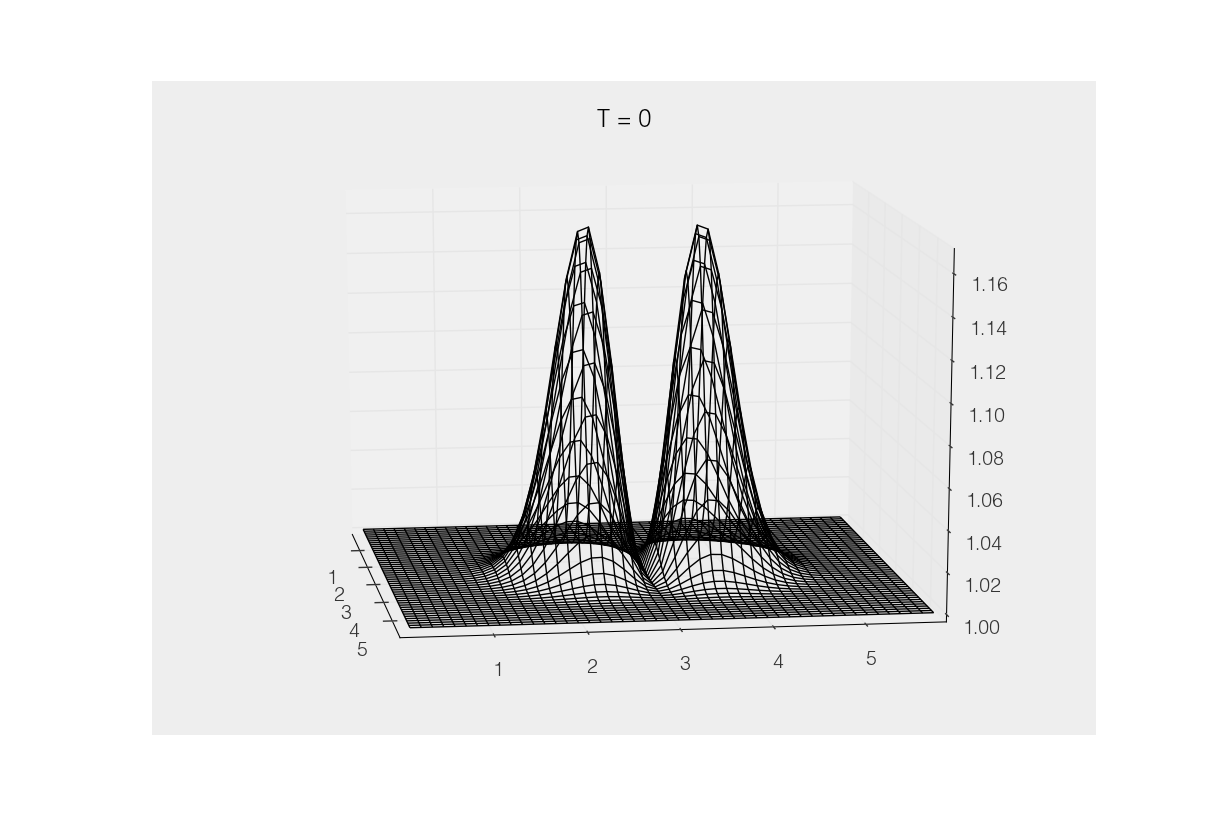
\includegraphics[width=\textwidth]{wirepertinit}
    \caption{}
    \label{fig:pert3}
  \end{subfigure}
  ~
  \begin{subfigure}[b]{0.48\textwidth}
    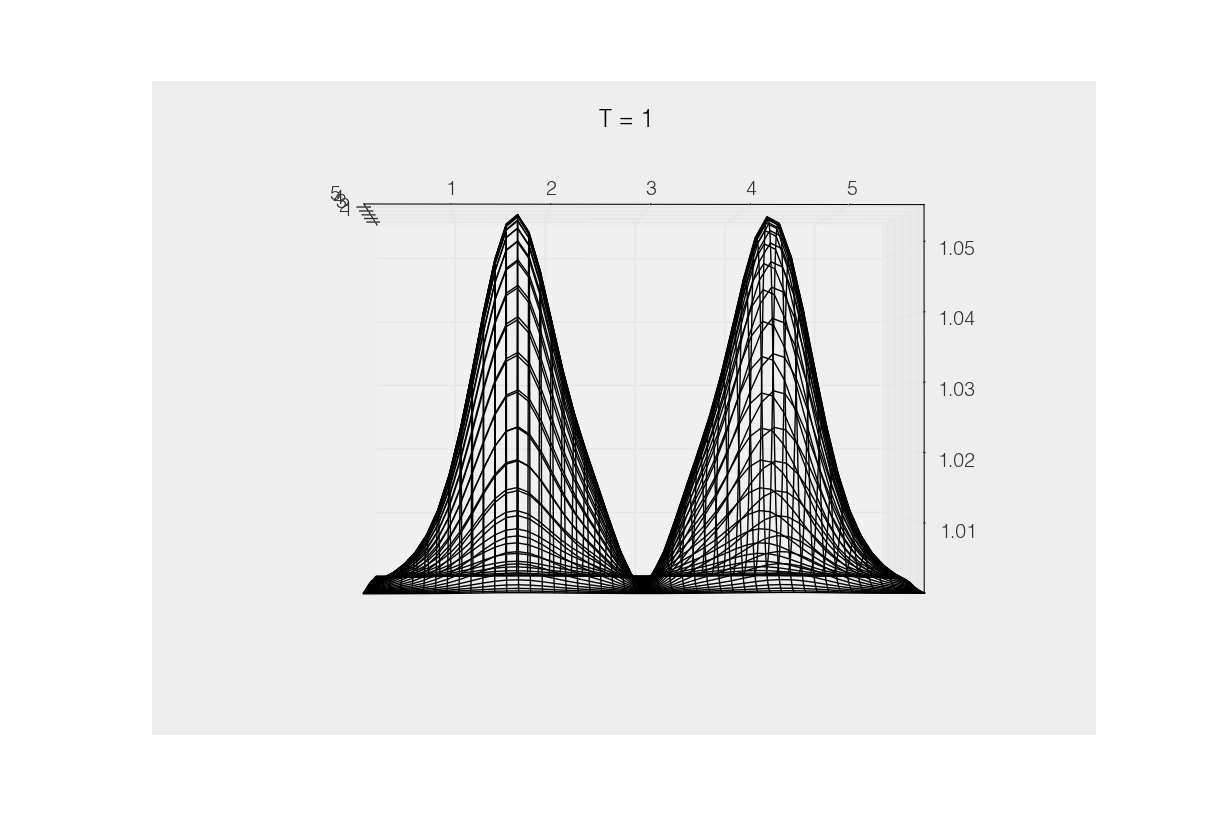
\includegraphics[width=\textwidth]{wirepert1}
    \caption{}
    \label{fig:pert4}
  \end{subfigure}
  \caption{Time evolution of a gaussian centered in a 2-D harmonic oscillator potential. (a),(c) show initial conditions. (b),(d) show time evolution after T=1. 50x50 grid, see Listing~\ref{schrodcode}}
  \label{fig:pert}
\end{figure}



\bibliographystyle{plain}
\bibliography{references}

\appendix

\section{Source Code}
\label{sec:code}

\lstinputlisting[label=heatcode,caption=Code to solve the heat equation]{adicart.c}
\lstinputlisting[label=lapcode,caption=Code to relex Laplace Equation]{adirelax.c}
\lstinputlisting[label=schrodcode,caption=Code to solve Schr\"{o}dinger Equation]{schrod.c}
 


\end{document}